\subsection{Improvements in the numerical algorithm}\label{numimprov}
The evaluation of integrals such as (\ref{eq:expval}) requires a way to sample the most relevant configurations (the \textit{typical set}) out of the entirety of parameter space. The simplest algorithm based on Markov chains for doing so is Metropolis-Hastings \cite{hastings}. Two crucial shortcomings of Metropolis are a rather slow exploration of the typical set based on a random walk in parameter space, and the large correlation between adjacent samples. A more sophisticated approach is Hybrid Monte Carlo, or HMC \cite{duane}: originally developed for lattice QCD computations, it allows a faster and more uniform exploration of the typical set by transposing the problem of sampling from a distribution to Hamiltonian evolution in a fictitious phase space.\newline
After a brief explanation of the idea behind HMC, the adaptation to the fuzzy space path integral is discussed and the results from numerical simulations are presented with a comparison between HMC and Metropolis.

\subsubsection{Hybrid Monte Carlo}
In Markov chain theory one is interested in a system specified by a finite set of parameters $(q_1, \cdots, q_N), \ q_i \in \mathbb{R}$, collectively referred to as $\mathbf{q}$. The probability that the system be in a particular configuration is given by some probability measure $\pi (\mathbf{q}) d\mathbf{q}$. Given an initial configuration $\mathbf{q}$, a Markov chain establishes a transition $\mathbf{q} \rightarrow \mathbf{q}'$ from the old configuration to a new one in such a way that $\mathbf{q}'$ is chosen with the desired probability.\newline 
This situation is analogous to the Monte Carlo estimation of the integral (\ref{eq:expval}), where the parameters are the independent degrees of freedom of the Dirac operator and the probability measure is $e^{-S[D]}dD$.\newline
The first step of Hybrid Monte Carlo is to enlarge parameter space by introducing a ``conjugate momentum'' $p_i$ to each parameter $q_i$, thus effectively working in a fictitious phase space. The probability measure is extended to include the new variables $\pi (\mathbf{q}) \rightarrow \pi (\mathbf{q}, \mathbf{p})$. By defining the ``Hamiltonian'' $H(\mathbf{q}, \mathbf{p}) \equiv -\log \pi (\mathbf{q}, \mathbf{p})$, a configuration is then evolved along a Hamiltonian trajectory by integrating Hamilton's equations:
\begin{align}
\frac{dq_i}{dt} &= \frac{\partial{H}}{\partial{p_i}} \label{eq:dqdt} \\
\frac{dp_i}{dt} &= -\frac{\partial{H}}{\partial{q_i}} \label{eq:dpdt}
\end{align}
where $t$ denotes a fictitious time that will be referred to as Monte Carlo time. This specifies a transition $(\mathbf{q}(0), \mathbf{p}(0)) \rightarrow (\mathbf{q}(t), \mathbf{p}(t))$ from an initial configuration to a new one. The new configuration is then accepted with probability $\text{min}[1, \exp (H(t)-H(0))]$. \newline
Note that Hamiltonian dynamics preserves the value of the energy of the system, therefore $H(t) = H(0)$ and $\text{min}[1, \exp (H(t)-H(0))] = 1$. However, numerical integration of Hamilton's equations is a non-trivial matter that introduces errors, therefore $H(t) \neq H(0)$ in general. The standard choice of numerical integrator in HMC is the so-called \textit{leapfrog} integrator \cite{neal} \cite{betan}.

\subsubsection{Adapting HMC to fuzzy spaces}
In the matrix integral considered here, the dynamical variables are the $n \times n$ Hermitian matrices $M_i$, to which a corresponding set of Hermitian matrices $P_i$ is added. The Hamiltonian is chosen to be simply:
\begin{equation} \label{eq:hamilt}
H(M_i, P_i) = S[M_i] + \sum_i \frac{1}{2}P_i^2.
\end{equation}
Schematically, the algorithm goes as follows:
\begin{enumerate}
\item extract the momenta $P_i$ according to $\exp(-P_i^2 / 2)$;
\item integrate Hamilton's equations for a certain time $t$;
\item accept the new configuration with probability $\text{min}[1, \exp (H(t)-H(0))]$.
\end{enumerate}
The non-trivial step in the leapfrog integrator is the evaluation of the force term in Eq.(YYYY), which requires to take derivatives such as:
\begin{equation}
\frac{\partial S[M_i]}{\partial M_k}
\end{equation}
which amounts to finding formulas for terms like:
\begin{equation}
\frac{\partial \Tr D(M_i)^p}{\partial M_k}.
\end{equation}
For the definition of matrix derivative see Appendix B. In the following, formulas for $p=2$ and $p=4$ are developed.

\subsubsection{The case $p=2$}
When $p = 2$ the $M_i$ matrices are decoupled:
\begin{equation}
\Tr D^2 = \sum_i \Tr \omega_i^2 (2 n \Tr M_i^2 + 2 \epsilon_i (\Tr M_i)^2).
\end{equation} 
Taking a derivative with respect to $M_k$ yields:
\begin{align}\label{eq:As}
\frac{\partial}{\partial M_k} \left( \sum_i \Tr \omega_i^2 (2 n \Tr M_i^2 + 2 \epsilon_i (\Tr M_i)^2) \right) = \notag \\
\sum_i \delta_{ik} \Tr \omega_i^2 \left( 4 n M_i^T + 4 \epsilon_i (\Tr M_i) I \right) = \notag \\
4 C \left( n M_k^T + \epsilon_k (\Tr M_k) I \right)
\end{align}
where $C \equiv \Tr \omega_i^2$ is the dimension of the Clifford module.

\subsubsection{The case $p=4$}
First expand $\Tr D^4$:
\begin{align}\label{eq:trd4}
\Tr D^4 &= \sum_{i_1, i_2, i_3, i_4} \Tr (\omega_{i_1} \omega_{i_2} \omega_{i_3} \omega_{i_4}) \cdot \notag \\
\Big( \ &n [1+\epsilon \ *] \Tr (M_{i_1} M_{i_2} M_{i_3} M_{i_4})  \ \  + \notag \\
&\epsilon_{i_1} \Tr M_{i_1} [1 + \epsilon \ *] \Tr ( M_{i_2} M_{i_3} M_{i_4})  \ \  + \notag \\
&\epsilon_{i_2} \Tr M_{i_2} [1  + \epsilon \ *] \Tr (M_{i_1} M_{i_3} M_{i_4}) \ \  + \notag \\
&\epsilon_{i_3} \Tr M_{i_3} [1 + \epsilon \ *] \Tr (M_{i_1} M_{i_2} M_{i_4})  \ \  + \notag \\
&\epsilon_{i_4} \Tr M_{i_4} [1 + \epsilon \ *] \Tr (M_{i_1} M_{i_2} M_{i_3})  \ \  + \notag \\
&\epsilon_{i_1} \epsilon_{i_2} [1 + \epsilon] \Tr (M_{i_1} M_{i_2} ) \Tr (M_{i_3} M_{i_4})   \ \  + \notag \\
&\epsilon_{i_1} \epsilon_{i_3} [1 + \epsilon] \Tr (M_{i_1} M_{i_3}) \Tr (M_{i_2} M_{i_4})   \ \  + \notag \\
&\epsilon_{i_1} \epsilon_{i_4} [1 + \epsilon] \Tr (M_{i_1} M_{i_4}) \Tr (M_{i_2} M_{i_3})   \ \Big)
\end{align}
where $*$ denotes complex conjugation of everything that appears on the right, $\epsilon$ is defined as the product $\epsilon \equiv \epsilon_{i_1}\epsilon_{i_2}\epsilon_{i_3}\epsilon_{i_4}$, and the relation $M^T = M^*$ has been used. Since $D$ is Hermitian, the expression must be real. It is not immediate to see that this is the case because of the $\epsilon = \pm 1$ factor inside the square brackets. Reality nonetheless holds, and becomes manifest by observing that a simultaneous index exchange $i_1 \leftrightarrow i_4$ and $i_2 \leftrightarrow i_3$ is equivalent to taking the complex conjugate (in fact, this is not the only index exchange that amounts to complex conjugation). \newline
Taking a matrix derivative with respect to $M_k$ results in non-vanishing contributions when $k=i_1, k=i_2, k=i_3$ or $k=i_4$:
\begin{align}
\frac{\partial}{\partial M_k} \Tr D^4 &= \sum_{i_1, i_2, i_3, i_4} \Tr (\omega_{i_1} \omega_{i_2} \omega_{i_3} \omega_{i_4}) \cdot \notag \\
\Big( &\delta_{ki_1} A(i_1, i_2, i_3, i_4)^T + \delta_{ki_2} A(i_2, i_3, i_4, i_1)^T + \notag \\
&\delta_{ki_3} A(i_3, i_4, i_1, i_2)^T + \delta_{ki_4} A(i_4, i_1, i_2, i_3)^T \Big)
\end{align}
where $A(a, b, c, d )$ is the following $n \times n$ matrix:
\begin{align}
A(a,b,c,d) \equiv \ &n [1+\epsilon \ \dagger] M_b M_c M_d + \notag \\
&\epsilon_a I [1 + \epsilon \ *] \Tr M_b M_c M_d  + \notag \\
&\epsilon_b \Tr M_b [1 + \epsilon \ \dagger] M_c M_d + \notag \\
&\epsilon_c \Tr M_c [1 + \epsilon \ \dagger] M_b M_d + \notag \\
&\epsilon_d \Tr M_d [1 + \epsilon \ \dagger] M_b M_c + \notag \\
&\epsilon_a \epsilon_b M_b [1 + \epsilon] \Tr M_c M_d + \notag \\
&\epsilon_a \epsilon_c M_c [1 + \epsilon] \Tr M_b M_d + \notag \\
&\epsilon_a \epsilon_d M_d [1 + \epsilon] \Tr M_b M_c
\end{align}
and $\dagger$ denotes Hermitian conjugation of everything that appears on the right. Upon relabeling the indices and cycling the $\omega$ matrices in the trace, the equation becomes:
\begin{align}\label{eq:derd4}
\frac{\partial}{\partial M_k} \Tr D^4 &= 4 \sum_{i_1, i_2, i_3, i_4} \delta_{ki_1} \Tr (\omega_{i_1} \omega_{i_2} \omega_{i_3} \omega_{i_4}) A(i_1, i_2, i_3, i_4)^T \notag \\
&= 4 \sum_{i_1, i_2, i_3} \Tr (\omega_{k} \omega_{i_1} \omega_{i_2} \omega_{i_3}) A(k, i_1, i_2, i_3)^T \equiv 4 \sum_{i_1, i_2, i_3} \mathcal{B}_k(i_1, i_2, i_3)
\end{align}
with $\mathcal{B}_k(a, b, c)$ denoting the generic term in the sum.\newline
To see that Eq.(\ref{eq:derd4}) defines a Hermitian matrix, notice that an exchange of indices $i_1 \leftrightarrow i_3$ is equivalent to taking the Hermitian conjugate:
\begin{equation}\label{eq:BBd}
\mathcal{B}_k(i_1, i_2, i_3)^{\dagger} = \mathcal{B}_k(i_3, i_2, i_1)
\end{equation}
therefore the sum in Eq.(\ref{eq:derd4}) reduces to:
\begin{equation}\label{eq:splitsum}
\sum_{\substack{i_1 > i_3 \\ i_2}} [1+\dagger] \mathcal{B}_k(i_1, i_2, i_3) + \sum_{i_1, i_2} \mathcal{B}_k(i_1, i_2, i_1).
\end{equation}
In fact, by looking at the form of $\mathcal{B}$, it is clear that terms in the sum are qualitatively different based on the number of indices that coincide. Therefore it would be computationally convenient to write Eq.(\ref{eq:splitsum}) in a way that emphazises this difference.\newline
The only terms that contribute when all indices are different are the following:
\begin{equation} \label{eq:alldifferent}
\sum_{i_1 > i_2 > i_3} [1+\dagger] \Big( \mathcal{B}_k(i_1, i_2, i_3) + \mathcal{B}_k(i_1, i_3, i_2) + \mathcal{B}_k(i_2, i_1, i_3) \Big).
\end{equation}
The three inequivalent permutations of indices that appear in this formula are based on a group-theoretical argument that will generalize easily to powers of $D$ higher than 4. First consider the symmetric group of order three $S_3$ acting on the set of indices $\{i_1, i_2, i_3\}$, and the subgroup of permutations that induce a simple change in $\mathcal{B}$, which in this case is $H = \{(), (13)\} \cong S_2$ (the first element being the identical permutation, and the second the exchange $i_1 \leftrightarrow i_3$ which induces $\mathcal{B} \rightarrow \mathcal{B}^\dagger$). The idea is then to restrict the sum to $i_1 > i_2 > i_3$ and quotient out the action of $H$ by introducing a suitable pre-factor that accounts for it (in this case $[1+\dagger]$). Practically, the inequivalent permutations of indices that appear in Eq.(\ref{eq:alldifferent}) are found by computing the (left or right) cosets of $H \subset S_3$ and acting on $\{i_1, i_2, i_3\}$ with a representative from each coset. In this case the representatives where chosen to be $(), (23), (12)$.\newline
What is left are terms in which at least two indices are equal. These are:
\begin{align} \label{eq:someequal}
\sum_{i_1 > i_2} [1+\dagger] \Big( \mathcal{B}_k(i_1, i_1, i_2) &+ \mathcal{B}_k(i_1, i_2, i_2) \Big) + \notag \\
&\sum_{i_1 \neq i_2} \mathcal{B}_k(i_1, i_2, i_1) + \sum_{i} \mathcal{B}_k(i,i,i).
\end{align}
At this point, a useful property of the $\omega$ matrices can be exploited to simplify both Eq.(\ref{eq:alldifferent}) and Eq.(\ref{eq:someequal}):
\begin{equation}\label{eq:gamma0}
\Tr(\omega_{\sigma(i_1)} \omega_{\sigma(i_2)} \omega_{\sigma(j)} \omega_{\sigma(k)}) \propto \Tr(\omega_j \omega_k) = 0 \qquad \text{if} \ \ i_1 = i_2 \ \text{and} \ j \neq k
\end{equation}
for any permutation $\sigma$ acting on $\{i_1, i_2, j, k\}$. In other words, if two indices are the same and the other two are different, the trace on the $\omega$ matrices vanishes.\newline
Putting together Eq.(\ref{eq:alldifferent}), Eq.(\ref{eq:someequal}) and Eq.(\ref{eq:gamma0}), the final formula for $\partial_k \Tr D^4$ reads:
\begin{align} 
\frac{\partial}{\partial M_k} \Tr D^4 = 4 \Bigg[ \sum_{\substack{i_1 > i_2 > i_3 \\ i_1,i_2,i_3 \neq k}} &[1+\dagger] \Big( \mathcal{B}_k(i_1, i_2, i_3) + \mathcal{B}_k(i_1, i_3, i_2) + \mathcal{B}_k(i_2, i_1, i_3) \Big) \notag \\
&+ \sum_{\substack{i \\ i \neq k}} \Big( [1+\dagger] \mathcal{B}_k(i, i, k) + \mathcal{B}_k(i, k, i) \Big) + \mathcal{B}_k(k,k,k) \Bigg].
\end{align}
The explicit form of $\mathcal{B}_k(i,i,k), \ \mathcal{B}_k(i,k,i)$ and $\mathcal{B}_k(k,k,k)$ is given in Appendix C.

\subsubsection{Testing HMC against exact results}
Although not many analytical results are available for the matrix integrals considered here, there is a non-trivial observable whose expectation value is known exactly for any geometry and any action polynomial in $D$. Computing this observable therefore provides a good test for the numerical implementation.\newline
Consider the following vanishing integral:
\begin{equation} \label{eq:vanint}
0 = \int \frac{\partial}{\partial D_{ij}} \left( D_{ij} e^{-S[D]} \right) d D
\end{equation}
where $D_{ij}$ is one of the independent degrees of freedom of the Dirac operator and $S[D]$ is in general sum of terms like $g_p \Tr D^p$.\newline
An explicit calculation of the right-hand side of Eq.(\ref{eq:vanint}) gives:
\begin{equation}
0 = \int \left( 1 - \sum_p g_p D_{ij} \frac{\partial}{\partial D_{ij}} \Tr D^p \right) e^{-S[D]}d D
\end{equation}
dividing by the partition function and rearranging the terms:
\begin{equation}
1 =\frac{1}{\int e^{-S[D]}} \int \left( \sum_p g_p D_{ij} \frac{\partial}{\partial D_{ij}} \Tr D^p \right) e^{-S[D]}d D
\end{equation}
and finally summing over all $i, j$ corresponding to independent degrees of freedom:
\begin{equation}\label{eq:dofs}
\#\text{d.o.f.}(D) = \frac{1}{\int e^{-S[D]}} \int \left( \sum_p g_p \ p \Tr D^p \right) e^{-S[D]} d D = \left\langle \sum_p g_p \ p \  \Tr D^p \right\rangle
\end{equation}
where the following identity, a proof of which is given in Appendix D, was used:
\begin{equation}
\sum_{ij} D_{ij} \frac{\partial}{\partial D_{ij}} \Tr D^p = p \Tr D^p.
\end{equation}
To estimate the number of degrees of freedom recall that in the decomposition (\ref{eq:dirac}) the $M_i$ matrices are all Hermitian, therefore {\#}d.o.f.$(D) = n^2m$ where $n$ is the dimension and $m$ the total number of $M_i$ matrices.\newline
Numerical tests of HMC and Metropolis agree with the prediction (\ref{eq:dofs}). As an example, a test on the $(0,3)$ Dirac operator is reported in Fig.(\ref{fig:dofs}).
\begin{figure}[hp]
\centering
\textbf{$\text{\# dofs} = 2 g_2 \langle S_2 \rangle + 4\langle S_4 \rangle$ test: comparison Metropolis/HMC}
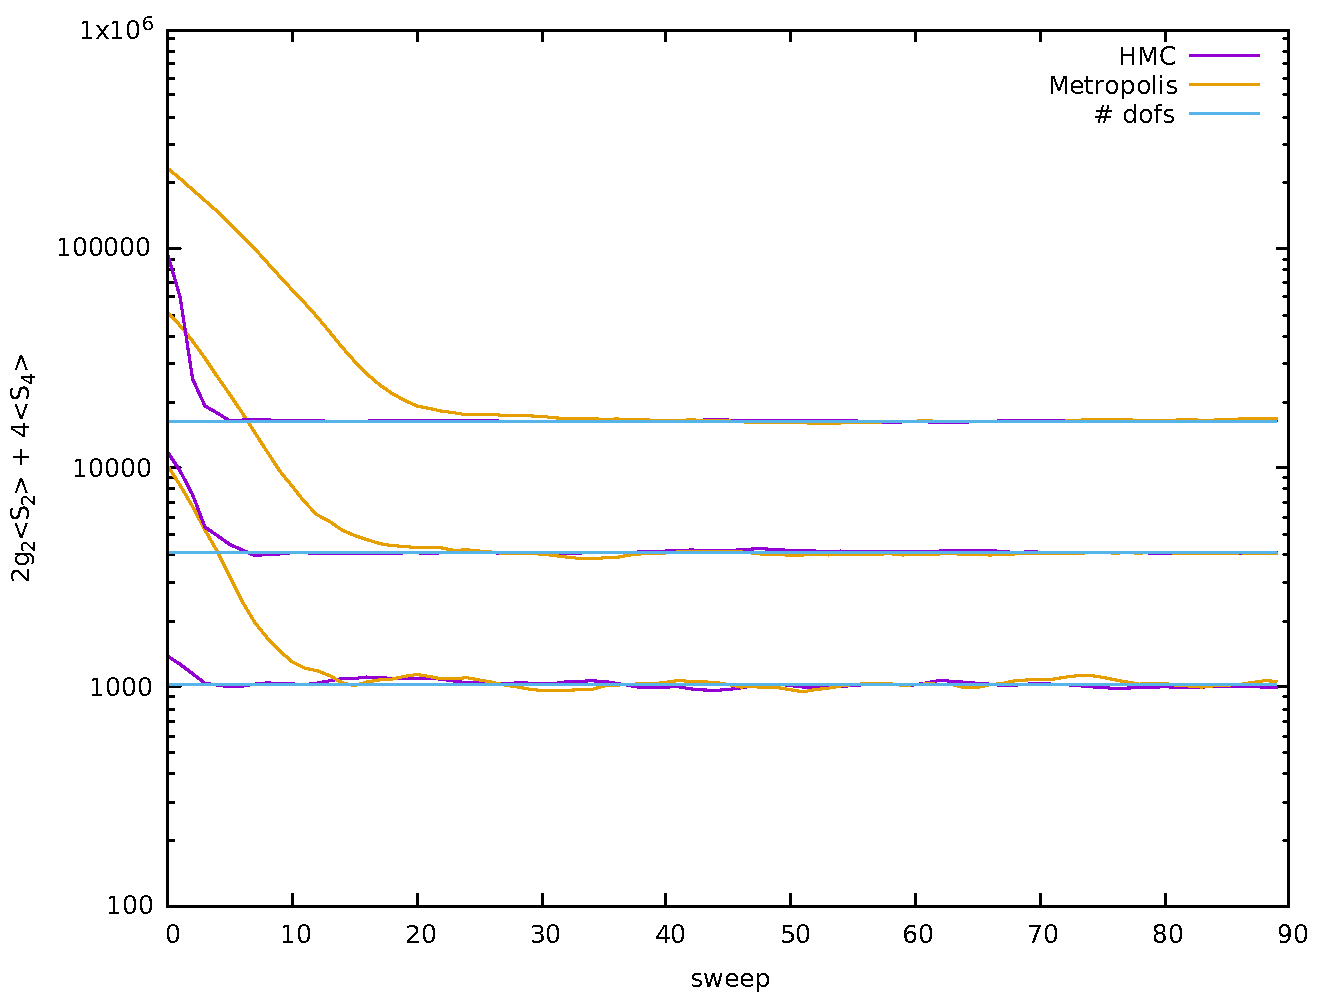
\includegraphics[width=1\linewidth]{fig/dofsp0q3.pdf}
\caption{Convergence of the expectation value of the observable $2 g_2 \Tr D^2 + 4 \Tr D^4 $ to the number of degrees of freedom of the Dirac operator for geometry $(0,3)$. The three sets correspond to matrix size $n = 16 \times 16$, $32 \times 32$ and $64 \times 64$. }
\label{fig:dofs}
\end{figure}

\subsubsection{Comparing the speed of HMC and Metropolis}
The samples produced by a Markov chain are correlated with each other. In general HMC generates less correlated samples if compared to Metropolis, resulting in higher quality data for a given computational cost.\newline
When computing a specific observable $O$, the efficiency of an algorithm in producing uncorrelated samples can be quantified by the \textit{time-displaced autocorrelation}:
\begin{equation}
\chi(t) = \int dt' O(t')O(t'+t) - \langle O \rangle^2
\end{equation}
where $O(t)$ represents the value of the observable at Monte Carlo time $t$. The autocorrelation function is expected to fall off exponentially:
\begin{equation}
\chi(t) \sim e^{-\frac{t}{\tau}}
\end{equation}
and $\tau$ is known as the autocorrelation time. Two values of the observable taken at $\sim 2\tau$ distance from each other are considered independent.\newline
The autocorrelation time tends to be dramatically larger near second-order phase transitions. For this reason the $(2,0)$ geometry at the phase transition was chosen to test HMC against Metropolis. The order parameter for the phase transition is:
\begin{equation}
F = \frac{(\Tr H_1)^2 + (\Tr H_2)^2}{n( \Tr H_1^2 + \Tr H_2^2)}
\end{equation}
where $H_i$ are the two free Hermitian matrices of the model. The plot of the time-displaced autocorrelation and the exponential fit for HMC and Metropolis are reported in Fig.(\ref{fig:autoc}). The exponential fit gives an autocorrelation time of $\sim 250$ sweeps for Metropolis and $\sim 25$ sweeps for HMC, meaning that in this example Metropolis needs to run 10 times longer than HMC for collecting the same amount of independent samples.
\begin{figure}[hp]
\centering
\textbf{Autocorrelation of order parameter $(2,0)$ test: comparison Metropolis/HMC}
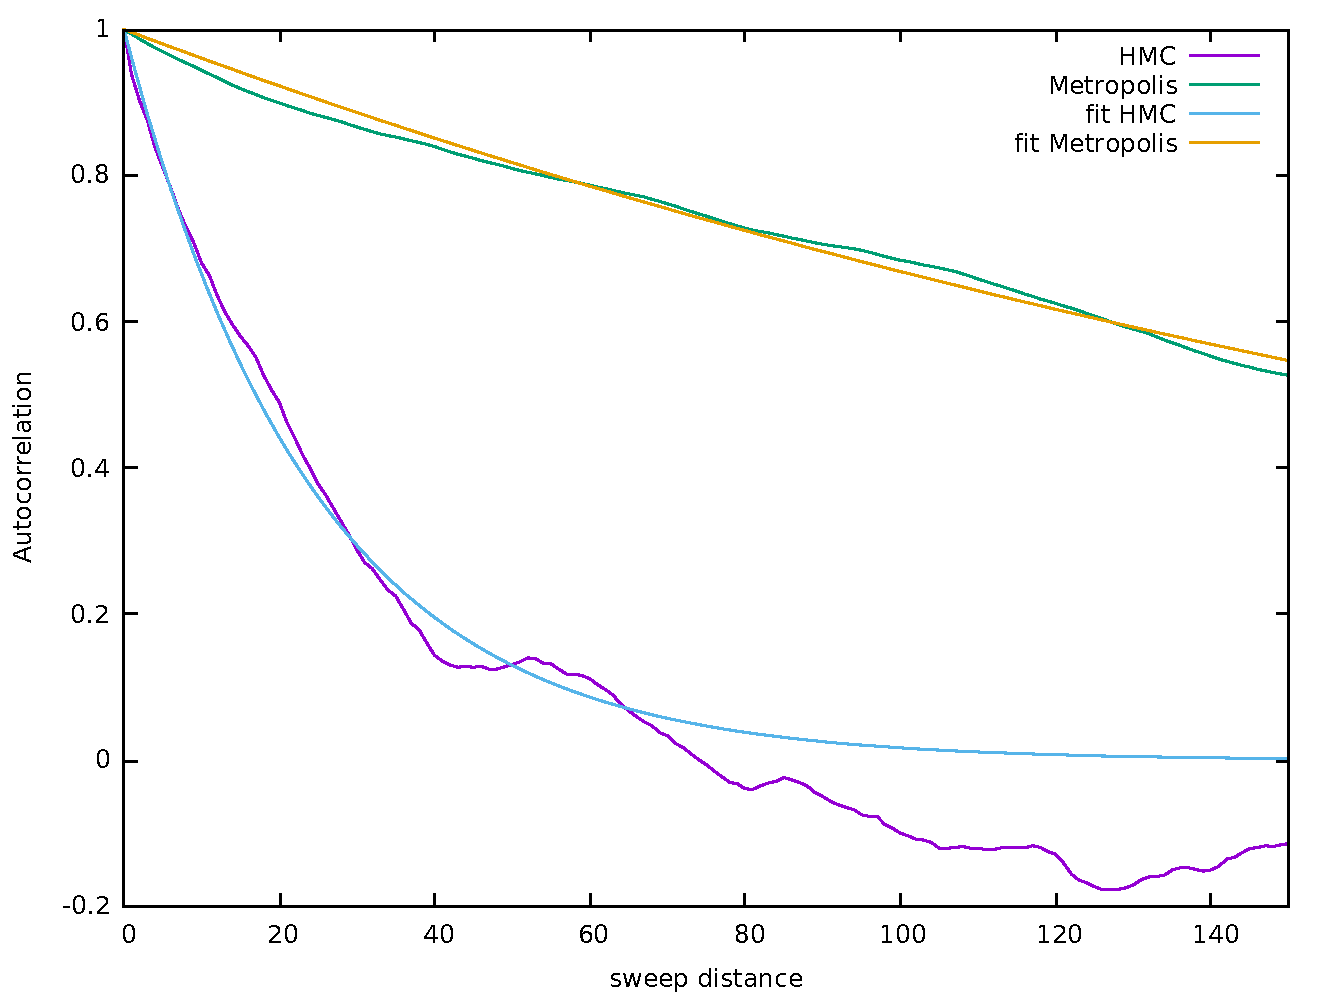
\includegraphics[width=1\linewidth]{fig/autocorrp2q0.pdf}
\caption{Autocorrelation $\chi (t)$ (normalized by $\chi(0)$) of the $(2,0)$ phase transition order parameter $F$. The coupling constant $g_2 = 2.725$ was chosen to be at the phase transition. The exponential fit gives an autocorrelation time of $\sim 250$ sweeps for Metropolis and $\sim 25$ sweeps for HMC.}
\label{fig:autoc}
\end{figure}
\newline
Of course Metropolis might be more than 10 times faster than HMC to collect a single sample, therefore the raw speed of the algorithm needs to be taken into account as well. In order to test this, the speed of HMC and Metropolis in generating 100 samples for the $(0,3)$ geometry was recorder for matrix dimension $16 \times 16$, $32 \times 32$ and $64 \times 64$. The results are reported in Tab.(\ref{tab:speed}).\newline
For small matrix size the two algorithms are comparable in speed, while for larger matrices HMC greatly outperforms Metropolis. Linearly fitting the data in logaritmic scale allows to estimate how the two algorithms scale with the matrix dimension, giving a computational cost of $O(n^{4.6})$ and $O(n^{2.6})$ for Metropolis and HMC respectively.
\begin{table}[hp]
\centering
\begin{tabular}{|l|l|l|}
\hline
\begin{tabular}[c]{@{}l@{}}Matrix\\ dimension\end{tabular} & \begin{tabular}[c]{@{}l@{}}time\\ HMC (sec)\end{tabular} & \begin{tabular}[c]{@{}l@{}}time\\ Metropolis (sec)\end{tabular} \\ \hline
16 & 23 & 17 \\ \hline
32 & 100 & 428 \\ \hline
64 & 1612 & 21218 \\ \hline
\end{tabular}
\caption{Time for 100 sweeps of HMC and Metropolis for geometry $(0,3)$. Fitting of the data gives a computational cost of $O(n^{4.6})$ and $O(n^{2.6})$ for Metropolis and HMC respectively.}
\label{tab:speed}
\end{table}


